\documentclass[11pt]{article}
\usepackage[utf8]{inputenc}

% Default fixed font does not support bold face
\DeclareFixedFont{\ttb}{T1}{txtt}{bx}{n}{10} % for bold
\DeclareFixedFont{\ttm}{T1}{txtt}{m}{n}{10}  % for normal

% Custom colors
\usepackage{color}
\definecolor{deepblue}{rgb}{0,0,0.5}
\definecolor{deepred}{rgb}{0.6,0,0}
\definecolor{deepgreen}{rgb}{0,0.5,0}

\usepackage{listings}

% Python style for highlighting
\newcommand\pythonstyle{\lstset{
language=Python,
basicstyle=\ttm,
otherkeywords={self},             % Add keywords here
keywordstyle=\ttb\color{deepblue},
emph={MyClass,__init__},          % Custom highlighting
emphstyle=\ttb\color{deepred},    % Custom highlighting style
stringstyle=\color{deepgreen},
frame=tb,                         % Any extra options here
showstringspaces=false            % 
}}


% Python environment
\lstnewenvironment{python}[1][]
{
\pythonstyle
\lstset{#1}
}
{}

% Python for external files
\newcommand\pythonexternal[2][]{{
\pythonstyle
\lstinputlisting[#1]{#2}}}

% Python for inline
\newcommand\pythoninline[1]{{\pythonstyle\lstinline!#1!}}
\usepackage{graphicx}
\usepackage{titling}
\usepackage{array}
\newcolumntype{P}[1]{>{\centering\arraybackslash}p{#1}}
\newcolumntype{M}[1]{>{\centering\arraybackslash}m{#1}}
\setcounter{secnumdepth}{0}
\usepackage{caption}
\usepackage{subfig}
\usepackage{geometry}
\geometry{
	top=2cm,
	left=2cm,
	right=2cm
}
\usepackage{hyperref}
\hypersetup{
	colorlinks=true,
	urlcolor=blue,
}
\urlstyle{same}

\tolerance=1
\emergencystretch=\maxdimen
\hyphenpenalty=10000
\hbadness=10000

\preauthor{%
  \begin{center}
  \LARGE
  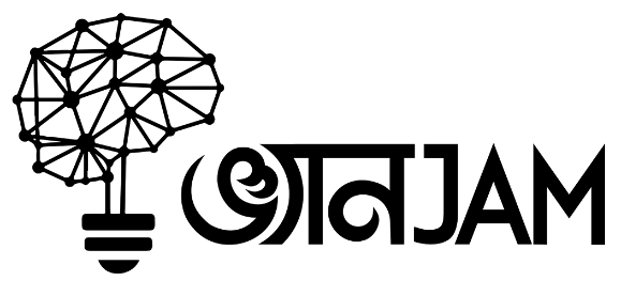
\includegraphics[scale=.4]{img/logo.png}\\[\bigskipamount]
}
\postauthor{\end{center}}
\title{Introduction to Machine Learning}
\date{}
\begin{document}
\maketitle
\section{Day 0}
\begin{enumerate}
\item Explain the difference between supervised and unsupervised machine
learning?\\[.5em]
In supervised machine learning algorithms, we have to provide labeled data, for example,
prediction of stock market prices, whereas in unsupervised we need not have labeled data, for example, classification of emails into spam and non-spam.

\item What Are the Applications of Supervised Machine Learning in Modern
Businesses?\\[.5em]
Applications of supervised machine learning include:
\begin{itemize}
\item \textbf{Email Spam Detection}\\
Here we train the model using historical data that consists of emails categorized as
spam or not spam. This labeled information is fed as input to the model.
\item \textbf{Healthcare Diagnosis}\\
By providing images regarding a disease, a model can be trained to detect if a person is
suffering from the disease or not.
\item \textbf{Sentiment Analysis}\\
This refers to the process of using algorithms to mine documents and determine
whether they’re positive, neutral, or negative in sentiment.
\item \textbf{Fraud Detection}\\
Training the model to identify suspicious patterns, we can detect instances of possible
fraud.
\end{itemize}

\item What Is Semi-supervised Machine Learning?\\[.5em]
Supervised learning uses data that is completely labeled, whereas unsupervised learning uses no training data. In the case of semi-supervised learning, the training data contains a small amount of labeled data and a large amount of unlabeled data.

\pagebreak
\item What are the different Algorithm techniques in Machine Learning?\\[.5em]
The different types of techniques in Machine Learning are:
\begin{itemize}
\item Supervised Learning
\item Unsupervised Learning
\item Semi-supervised Learning
\item Reinforcement Learning
\item Transduction
\item Learning to Learn
\end{itemize}

\item What Are Unsupervised Machine Learning Techniques?\\[.5em]
There are two techniques used in unsupervised learning: clustering and association.
\begin{itemize}
\item Clustering
\begin{itemize}
\item Clustering problems involve data to be divided into subsets. These subsets, also called
clusters, contain data that are similar to each other. Different clusters reveal different
details about the objects, unlike classification or regression.
\end{itemize}
\item Association
\begin{itemize}
\item In an association problem, we identify patterns of associations between different
variables or items.
\item For example, an eCommerce website can suggest other items for you to buy, based on
the prior purchases that you have made, spending habits, items in your wishlist, other
customers’ purchase habits, and so on.
\end{itemize}
\end{itemize}
\end{enumerate}
\pagebreak
\section{Day 1}
\begin{enumerate}
\item What is Jupyter Notebook?\\[.5em]
The Jupyter Notebook is an open-source web application that allows you to create and share documents that contain live code, equations, visualizations and narrative text. Uses include: data cleaning and transformation, numerical simulation, statistical modeling, data visualization, machine learning, and much more.

\item Write down the code for displaying $\sin{x}$ between $[0, 3\pi]$\\[.5em]
\begin{python}
import numpy as np 
import matplotlib.pyplot as plt  

# Compute the x and y coordinates for points on a sine curve 
x = np.arange(0, 3 * np.pi, 0.1) 
y = np.sin(x) 
plt.title("sine wave form") 

# Plot the points using matplotlib 
plt.plot(x, y) 
plt.show() 
\end{python}

\item Explain NumPy broadcasting.\\[.5em]
Broadcasting is the methodology adopted in NumPy used to perform arithmetic operations on arrays with differing dimensions. General arithmetic operations such as addition, multiplication, subtraction, etc. tend to broadcast arrays before performing the operations on arrays with variations in size.

\item What method would you use for creating a 3x5x6 random array of doubles?\\[.5em]
\begin{python}
numpy.random.randn(3,5,6)
\end{python}

\item How would you create a 3x6 matrix of zeros and ones?\\[.5em]
\begin{python}
numpy.zeros((3, 6), dtype=int)
numpy.ones((3, 6), dtype=int)
\end{python}
\end{enumerate}
\pagebreak
\section{Day 2}
\begin{enumerate}
\item What are the parametric models? Give an example.\\[.5em]
Parametric models are those with a finite number of parameters. To predict new data, you only
need to know the parameters of the model. Examples include linear regression, logistic
regression, and linear SVMs.

Non-parametric models are those with an unbounded number of parameters, allowing for more
flexibility. To predict new data, you need to know the parameters of the model and the state of
the data that has been observed. Examples include decision trees, k-nearest neighbors, and
topic models using latent Dirichlet analysis.

\item What is the difference between classification and regression?\\[.5em]
Classification is used to produce discrete results, classification is used to classify data into some
specific categories. For example, classifying emails into spam and non-spam categories.
Whereas, We use regression analysis when we are dealing with continuous data, for example
predicting stock prices at a certain point in time.

\item What is Linear Regression?\\[.5em]
Linear Regression is a supervised Machine Learning algorithm. It is used to find the linear
relationship between the dependent and the independent variables for predictive analysis.

\item What are the drawbacks of a linear model?\\[.5em]
There are a couple of drawbacks of a linear model:
\begin{itemize}

\item A linear model holds some strong assumptions that may not be true in the application. It
assumes a linear relationship, multivariate normality, no or little multicollinearity, no
auto-correlation, and homoscedasticity
\item A linear model can’t be used for discrete or binary outcomes.
\item You can’t vary the model flexibility of a linear model.
\end{itemize}

\item When does the linear regression line stop rotating or finds an optimal spot where it
is fitted on data?\\[.5em]
A place where the highest RSquared value is found, is the place where the line comes to rest.
RSquared represents the amount of variance captured by the virtual linear regression line with
respect to the total variance captured by the dataset.
\end{enumerate}
\pagebreak

\section{Day 3}
\begin{enumerate}
\item What Is Overfitting, and How Can You Avoid It?\\[.5em]
Overfitting is a situation that occurs when a model learns the training set too well, taking up
random fluctuations in the training data as concepts. These impact the model's ability to
generalize and don’t apply to new data.
When a model is given the training data, it shows 100 percent accuracy—technically a slight
loss. But, when we use the test data, there may be an error and low efficiency. This condition is
known as overfitting.
There are multiple ways of avoiding overfitting, such as:
\begin{itemize}
\item Regularization. It involves a cost term for the features involved with the objective function
\item Making a simple model. With lesser variables and parameters, the variance can be
reduced
\item Cross-validation methods like k-folds can also be used
\item If some model parameters are likely to cause overfitting, techniques for regularization
like LASSO can be used that penalize these parameters
\end{itemize}

\item When does regularization becomes necessary in Machine Learning?\\[.5em]
Regularization becomes necessary when the model begins to overfit/underfit. This technique
introduces a cost term for bringing in more features with the objective function. Hence, it tries to
push the coefficients for many variables to zero and hence reduce the cost term. This helps to
reduce model complexity so that the model can become better at predicting (generalizing).

\item What does the term decision boundary mean?\\[.5em]
A decision boundary or a decision surface is a hypersurface which divides the
underlying feature space into two subspaces, one for each class. If the decision boundary is a
hyperplane, then the classes are linearly separable.

\item How can learning curves help create a better model?\\[.5em]
Learning curves give the indication of the presence of overfitting or underfitting.

In a learning curve, the training error and cross-validating error are plotted against the number
of training data points.

\item What is the difference between stochastic gradient descent (SGD) and
gradient descent (GD)?\\[.5em]
Both algorithms are methods for finding a set of parameters that minimize a loss function by
evaluating parameters against data and then making adjustments.

In standard gradient descent, you'll evaluate all training samples for each set of parameters.
This is akin to taking big, slow steps toward the solution.

In stochastic gradient descent, you'll evaluate only 1 training sample for the set of parameters
before updating them. This is akin to taking small, quick steps toward the solution.
\end{enumerate}
\pagebreak

\section{Day 4}
\begin{enumerate}
\item What Is ‘naive’ in the Naive Bayes Classifier?\\[.5em]
The classifier is called ‘naive’ because it makes assumptions that may or may not turn out to be
correct.

The algorithm assumes that the presence of one feature of a class is not related to the presence
of any other feature (absolute independence of features), given the class variable.

For instance, a fruit may be considered to be a cherry if it is red in color and round in shape,
regardless of other features. This assumption may or may not be right (as an apple also
matches the description).

\item What Is Decision Tree Classification?\\[.5em]
A decision tree builds classification (or regression) models as a tree structure, with datasets
broken up into ever-smaller subsets while developing the decision tree, literally in a tree-like
way with branches and nodes. Decision trees can handle both categorical and numerical data.

\item What Is Pruning in Decision Trees, and How Is It Done?\\[.5em]
Pruning is a technique in machine learning that reduces the size of decision trees. It reduces the
complexity of the final classifier, and hence improves predictive accuracy by the reduction of
overfitting.

\item In k-means or KNN, we use euclidean distance to calculate the distance
between nearest neighbors. Why not manhattan distance?\\[.5em]
We don’t use manhattan distance because it calculates distance horizontally or vertically only. It
has dimension restrictions. On the other hand, the euclidean metric can be used in any space to
calculate distance. Since the data points can be present in any dimension, euclidean distance is
a more viable option.
\item What is a Decision Tree?\\[.5em]
A decision tree is used to explain the sequence of actions that must be performed to get the
desired output. It is a hierarchical diagram that shows the actions.
\end{enumerate}
\pagebreak

\section{Day 5}
\begin{enumerate}
\item Define Precision and Recall.\\[.5em]
Precision
\begin{itemize}
\item Precision is the ratio of several events you can correctly recall to the total number of
events you recall (mix of correct and wrong recalls).
\item Precision = (True Positive) / (True Positive + False Positive)
\end{itemize}
Recall
\begin{itemize}
\item A recall is the ratio of a number of events you can recall the number of total events.
\item Recall = (True Positive) / (True Positive + False Negative)
\end{itemize}

\item What is meant by ‘Training set’ and ‘Test Set’?\\[.5em]
We split the given data set into two different sections namely,’ Training set’ and ‘Test Set’.
‘Training set’ is the portion of the dataset used to train the model.

‘Testing set’ is the portion of the dataset used to test the trained model.

\item Explain the Bias-Variance Tradeoff.\\[.5em]
Predictive models have a tradeoff between bias (how well the model fits the data) and variance
(how much the model changes based on changes in the inputs).

Simpler models are stable (low variance) but they don't get close to the truth (high bias).

More complex models are more prone to overfitting (high variance) but they are expressive
enough to get close to the truth (low bias). The best model for a given problem usually lies
somewhere in the middle.

\item How much data should you allocate for your training, validation, and test
sets?\\[.5em]
You have to find a balance, and there's no right answer for every problem.

If your test set is too small, you'll have an unreliable estimation of model performance
(performance statistic will have high variance). If your training set is too small, your actual model
parameters will have a high variance.

A good rule of thumb is to use an 80/20 train/test split. Then, your train set can be further split
into train/validation or into partitions for cross-validation.

\item What Is a False Positive and False Negative and How Are They Significant?\\[.5em]
False positives are those cases which wrongly get classified as True but are False.
False negatives are those cases which wrongly get classified as False but are True.

In the term ‘False Positive,’ the word ‘Positive’ refers to the ‘Yes’ row of the predicted value in
the confusion matrix. The complete term indicates that the system has predicted it as a positive,
but the actual value is negative.
\end{enumerate}
\pagebreak

\section{Day 6}
\begin{enumerate}
\item What Is Kernel SVM?\\[.5em]
Kernel SVM is the abbreviated version of the kernel support vector machine. Kernel methods
are a class of algorithms for pattern analysis, and the most common one is the kernel SVM.

\item What are support vector machines?\\[.5em]
Support vector machines are supervised learning algorithms used for classification and
regression analysis.

\item When would you use random forests Vs SVM and why?\\[.5em]
There are a couple of reasons why a random forest is a better choice of the model than a
support vector machine:
\begin{itemize}
\item Random forests allow you to determine the feature importance. SVM’s can't do this.
\item Random forests are much quicker and simpler to build than an SVM.
\item For multi-class classification problems, SVMs require a one-vs-rest method, which is
less scalable and more memory intensive.
\end{itemize}

\item What is a kernel? Explain the kernel trick\\[.5em]
A kernel is a way of computing the dot product of two vectors xx and yy in some (possibly very
high dimensional) feature space, which is why kernel functions are sometimes called
“generalized dot product”

The kernel trick is a method of using a linear classifier to solve a non-linear problem by
transforming linearly inseparable data to linearly separable ones in a higher dimension.

\item How does the SVM algorithm deal with self-learning?\\[.5em]
SVM has a learning rate and expansion rate which takes care of this. The learning rate
compensates or penalises the hyperplanes for making all the wrong moves and expansion rate
deals with finding the maximum separation area between classes.
\end{enumerate}
\pagebreak

\section{Day 7}
\begin{enumerate}
\item Explain Principle Component Analysis (PCA).\\[.5em]
PCA is a method for transforming features in a dataset by combining them into uncorrelated
linear combinations.

These new features, or principal components, sequentially maximize the variance represented
(i.e. the first principal component has the most variance, the second principal component has
the second most, and so on).

\item What Are Some Methods of Reducing Dimensionality?\\[.5em]
You can reduce dimensionality by combining features with feature engineering, removing
collinear features, or using algorithmic dimensionality reduction.

Now that you have gone through these machine learning interview questions, you must have
got an idea of your strengths and weaknesses in this domain.

\item How is KNN different from k-means clustering?\\[.5em]
K-Nearest Neighbors is a supervised classification algorithm, while k-means clustering is an
unsupervised clustering algorithm. While the mechanisms may seem similar at first, what this
really means is that in order for K-Nearest Neighbors to work, you need labeled data you want
to classify an unlabeled point into (thus the nearest neighbor part). K-means clustering requires
only a set of unlabeled points and a threshold: the algorithm will take unlabeled points and
gradually learn how to cluster them into groups by computing the mean of the distance between
different points.

\item Why is the rotation of components so important in Principle Component
Analysis(PCA)?\\[.5em]
Rotation in PCA is very important as it maximizes the separation within the variance obtained by
all the components because of which interpretation of components would become easier. If the
components are not rotated, then we need extended components to describe the variance of
the components.

\item What are PCA, KPCA, and ICA used for?\\[.5em]
PCA (Principal Components Analysis), KPCA ( Kernel-based Principal Component Analysis)
and ICA ( Independent Component Analysis) are important feature extraction techniques used
for dimensionality reduction.
\end{enumerate}
\pagebreak

\section{Day 8}
\begin{enumerate}
\item How do you handle outliers in the data?\\[.5em]
Outlier is an observation in the data set that is far away from other observations in the data set.
We can discover outliers using tools and functions like box plot, scatter plot, Z-Score, IQR score
etc. and then handle them based on the visualization we have got. To handle outliers, we can
cap at some threshold, use transformations to reduce skewness of the data and remove outliers
if they are anomalies or errors.

\item Mention some of the EDA Techniques?\\[.5em]
Exploratory Data Analysis (EDA) helps analysts to understand the data better and forms the
foundation of better models.\\
\textbf{Visualization:-}
\begin{itemize}
\item Univariate visualization
\item Bivariate visualization
\item Multivariate visualization
\end{itemize}
\textbf{Missing Value Treatment} — Replace missing values with Either Mean/Median\\
\textbf{Outlier Detection} — Use Boxplot to identify the distribution of Outliers, then Apply IQR to set the
boundary for IQR

\item What are 3 data preprocessing techniques to handle outliers?
\begin{itemize}
\item Winsorize (cap at threshold).
\item Transform to reduce skew (using Box-Cox or similar).
\item Remove outliers if you're certain they are anomalies or measurement errors.
\end{itemize}

\item Generate a normal distribution array of size 2x3.\\[.5em]
\begin{python}
from numpy import random

x = random.normal(size=(2, 3))
\end{python}

\item Write down the code needed to visualize a Gaussian distribution.\\[.5em]
\begin{python}
from numpy import random
import matplotlib.pyplot as plt
import seaborn as sns

sns.distplot(random.normal(size=1000), hist=False)

plt.show()
\end{python}
\end{enumerate}
\pagebreak

\section{Day 9}
\begin{enumerate}
\item What Is a Recommendation System?\\[.5em]
Anyone who has used Spotify or shopped at Amazon will recognize a recommendation system:
It's an information filtering system that predicts what a user might want to hear or see based on
choice patterns provided by the user.

\item How would you implement a recommendation system for our company’s
users?\\[.5em]
A lot of machine learning interview questions of this type will involve the implementation of
machine learning models to a company’s problems. You'll have to research the company and its
industry in-depth, especially the revenue drivers the company has, and the types of users the
company takes on in the context of the industry it’s in.

\item Name and define techniques used to find similarities in the recommendation system.\\[.5em]
Pearson correlation and Cosine correlation are techniques used to find similarities in
recommendation systems.

\item What is Collaborative Filtering?\\[.5em]
Collaborative filtering is a technique that can filter out items that a user might like on the basis of reactions by similar users. It works by searching a large group of people and finding a smaller set of users with tastes similar to a particular user.

\item What are the steps involved in building a simple recommender system?\\[.5em]
The following are the steps involved:
\begin{itemize}
\item	 Decide on the metric or score to rate movies on.

\item Calculate the score for every movie.

\item Sort the movies based on the score and output the top results.
\end{itemize}
\end{enumerate}
\pagebreak

\section{Day 10}
Applied Machine Learning Project--\hspace{9cm}\textbf{20 Marks}\\
\vspace{5cm}
\begin{figure}[h!]
\centering
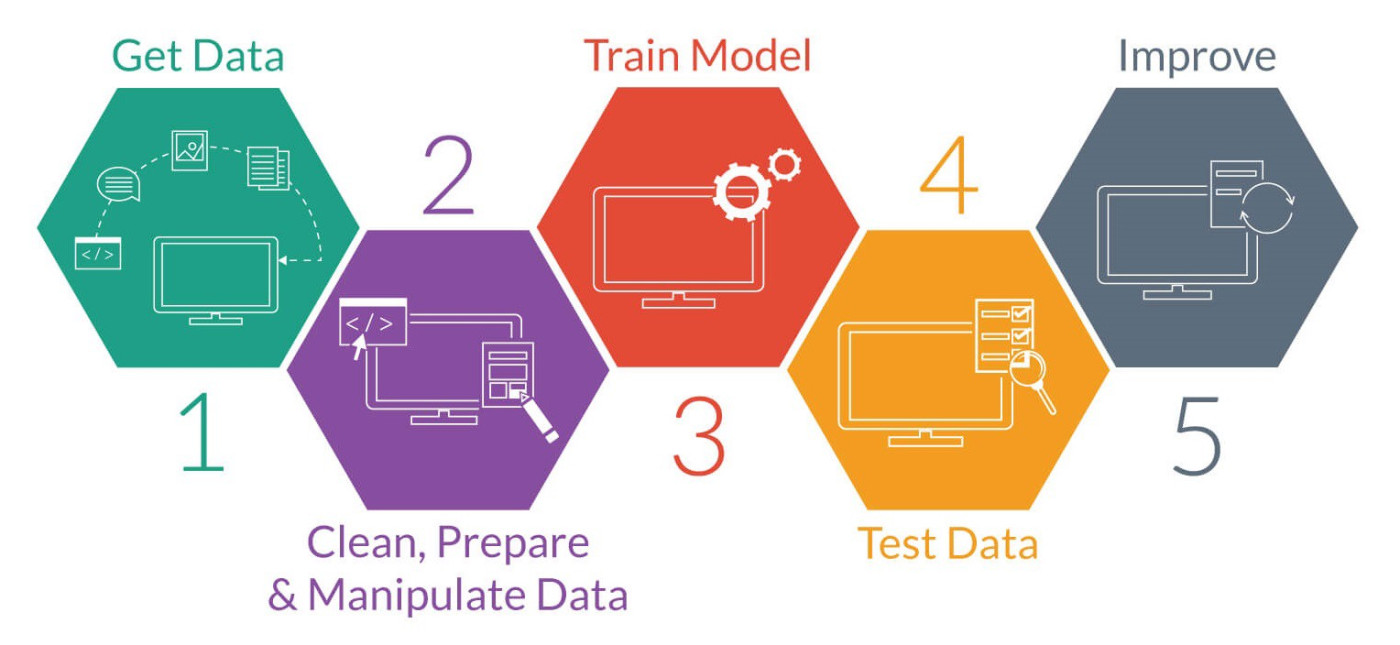
\includegraphics[scale=.3]{img/mlproj.jpeg}
\end{figure}
\pagebreak

\section{Day 11}
\begin{enumerate}
\item How Can You Choose a Classifier Based on a Training Set Data Size?\\[.5em]
When the training set is small, a model that has a right bias and low variance seems to work
better because they are less likely to overfit.

\item How Do You Handle Missing or Corrupted Data in a Dataset?\\[.5em]
One of the easiest ways to handle missing or corrupted data is to drop those rows or columns or
replace them entirely with some other value.
There are two useful methods in Pandas:
\begin{itemize}
\item IsNull() and dropna() will help to find the columns/rows with missing data and drop them
\item Fillna() will replace the wrong values with a placeholder value
\end{itemize}

\item What is deep learning, and how does it contrast with other machine learning
algorithms?\\[.5em]
Deep learning is a subset of machine learning that is concerned with neural networks: how to
use backpropagation and certain principles from neuroscience to more accurately model large
sets of unlabelled or semi-structured data. In that sense, deep learning represents an unsupervised learning algorithm that learns representations of data through the use of neural
nets.

\item When should you use classification over regression?\\[.5em]
Classification produces discrete values and dataset to strict categories, while regression gives
you continuous results that allow you to better distinguish differences between individual points.
You would use classification over regression if you wanted your results to reflect the
belongingness of data points in your dataset to certain explicit categories (ex: If you wanted to
know whether a name was male or female rather than just how correlated they were with male
and female names.)

\item Difference between machine learning and deep learning\\[.5em]
Machine learning is a branch of computer science and a method to implement artificial
intelligence. This technique provides the ability to automatically learn and improve from
experiences without being explicitly programmed.

Deep learning can be said as a subset of machine learning. It is mainly based on the artificial
neural network where data is taken as an input and the technique makes intuitive decisions
using the artificial neural network.
\end{enumerate}

\end{document}